\section{Motivation}
\label{sec:motivation}

\subsection{Illustrating scenario}

Consider a team of language designers working on the construction of the DSLs for state machines presented in section \ref{sec:background}. During that process, language designers implement the language constructs typically required for expressing finite state machines: states, transitions, events, and so on. In addition, the DSL is intended to provide a constraints language that allows final users to express guards on the transitions. Moreover, the DSL also provides an expressions language that allows to specify actions on the states of the state machine. This expressions language offers classical capabilities such as arithmetic operations, variables management, and imperative procedures. 

After being released their DSL for state machines, the language development team is required again. This time the objective is to build a DSL for manipulating the traditional Logo turtle which is often used in elementary schools for teaching the first foundations of programming \cite{Olson:1987}. Certainly, the new DSL is essentially different from the DSL for state machines. Instead of states and transitions, Logo offers some primitives (such as \texttt{Forward}, \texttt{Backward}, \texttt{Left}, and \texttt{Right}) to move a character (i.e., the turtle) within a bounded canvas. However, Logo also requires an expressions language in order to specify complex movements. For example, final users may write instructions such as: \texttt{forward (x + 2)} where \texttt{x} is a variable.

At this point, language designers face the question of how to reuse the expressions language they already defined for the state machines language. As illustrated in Figure \ref{fig:cloning}, the typical solution to this type of situations is to replicate the code in a second DSL. Language designers usually copy/paste the segment of the specification that they can reuse. As a result, we have many clones that are expensive to maintain. Naturally, this situation is repeated each time that there is a new DSL to build. This fact is illustrated in the Figure \ref{fig:cloning} by introducing a third DSL for expressing flowcharts. In this case, the new DSL requires both, expressions and constraints languages. 

\begin{figure}
\centering
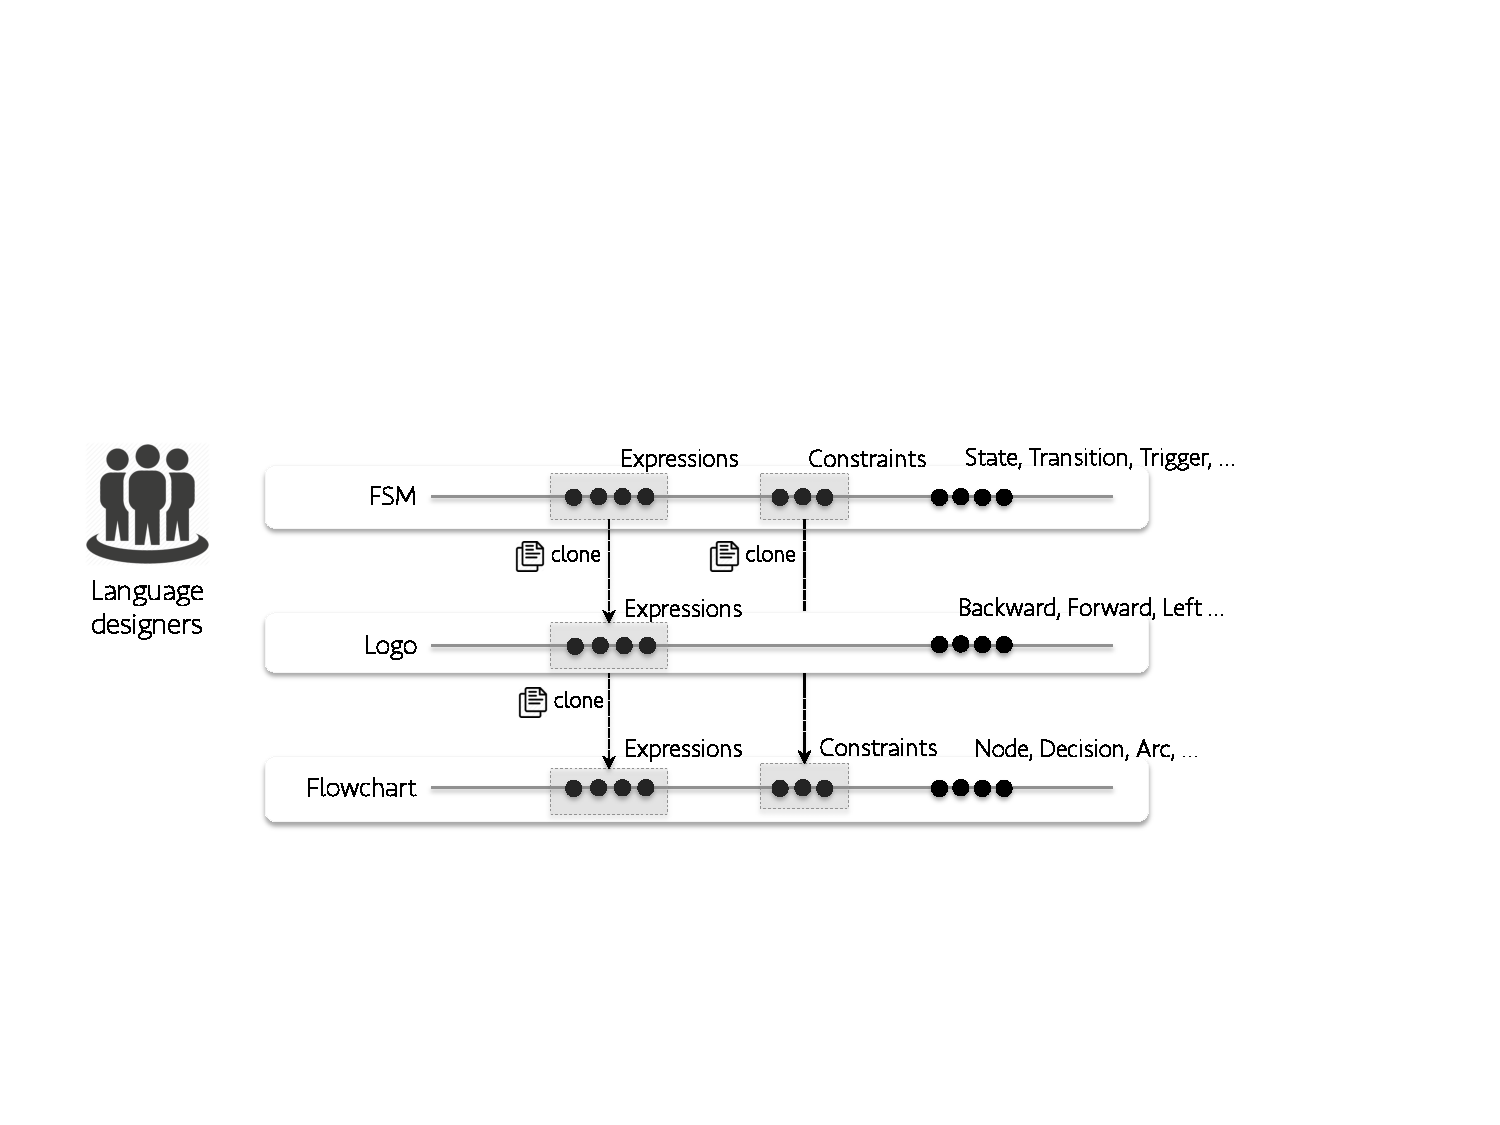
\includegraphics[width=1\linewidth]{images/cloning.pdf}
\caption{Cloning in DSLs development process}
\label{fig:cloning}
\end{figure}

%As a matter of fact, these DSLs are essentially different. Each of them is focus on a particular domain and offers different language constructs. However, there are syntactic and semantic commonalities that are illustrated in Figure \ref{fig:domains}. All the thee DSLs offer some expressions for modifying variables. In the case of FSM these actions are needed the specification of the actions in the states; in the case of Logo expressions are needed to specity the movement and rotation parameters; and in the case of flowchart expressions are needed to specify the body of actions. In addition, both FSM and Flowchart rely on a constraints language. The former for expressing guards in the transitions and the later for expressing guards of the decisions.

\subsection{Overlapping in DSLs and potential reuse}

The aforementioned phenomenon was previously observed by V\"oelter et al \cite[p. 60-61]{voelter:2013}. In fact, that study demonstrates that although many of the existing DSLs are completely different and tackle independent domains; there are related DSLs with overlapping domains. That is, they share certain language constructs i.e., they have \textbf{commonalities} between them. Figure \ref{fig:shape} illustrates this observation for the case of our illustrating scenario and by using two Venn diagrams to represent both syntax and semantic overlapping. Syntactic and semantic overlapping is represented as intersections between the corresponding sets. To this end, we designed an algorithm that is able to compute the all overlapping among the syntax of the DSLs in the input set. 

\begin{figure}
\centering
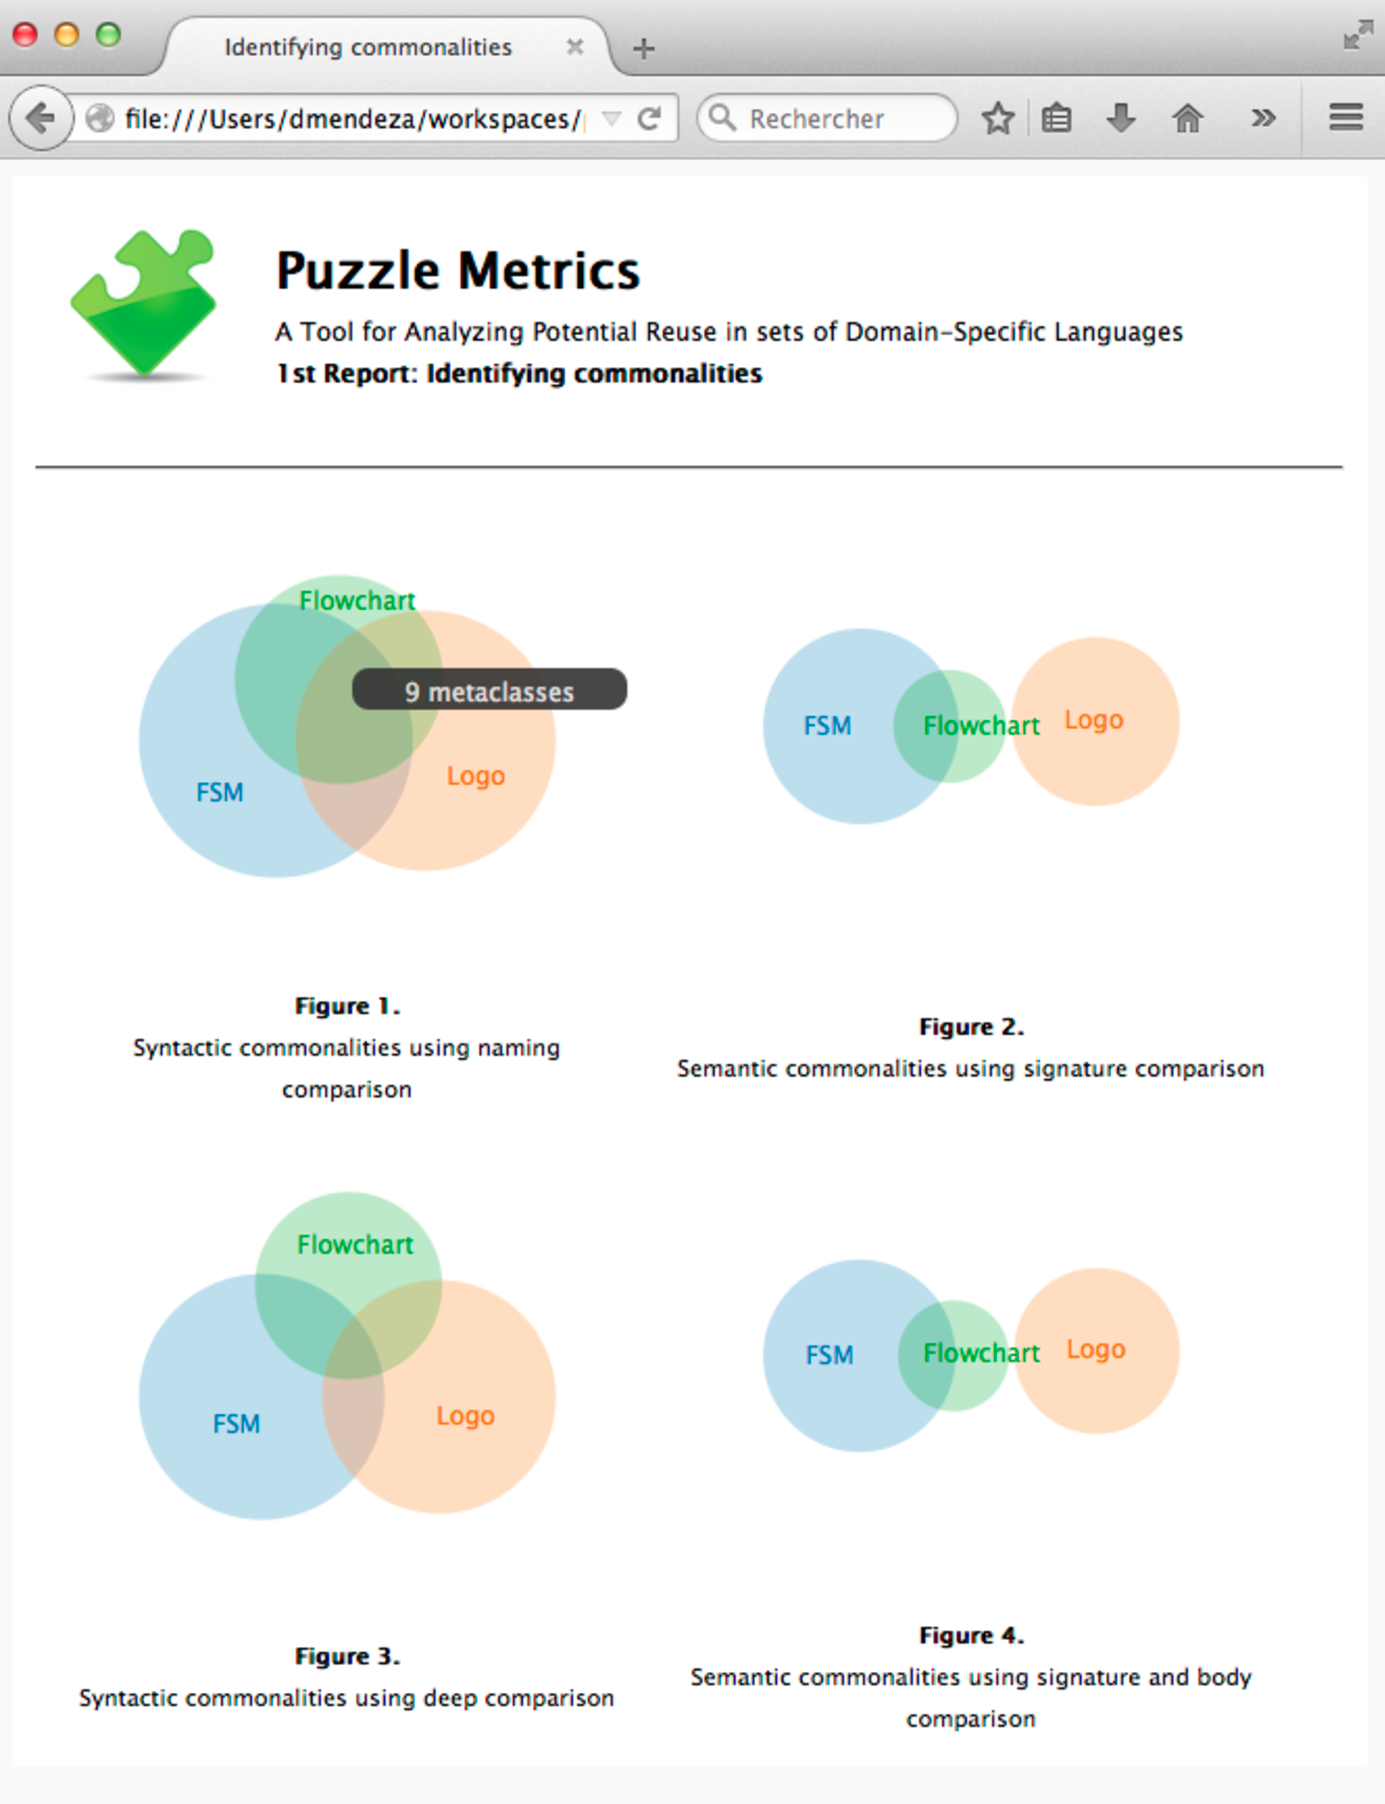
\includegraphics[width=1\linewidth]{images/domains-inaction.pdf}
\caption{Visualizing syntactic and semantic commonalities}
\label{fig:shape}
\end{figure}

If a set of DSLs have some overlapping and they are specified in the same technological space and using compatible language workbenches, then there is \textbf{potential reuse} since the specification of those shared constructs can be specified once and reused in the two DSLs \cite[p. 60-61]{voelter:2013}. For the technological space discussed in this paper, syntactic commonalities appear where DSLs share some metaclasses and semantic commonalities appear where DSLs share some domain-specific actions.

%Figure \ref{fig:domains} illustrates the phenomenon in our illustrating scenario. Note that each DSL is specified in terms of a set of metaclasses (top of the figure), and a set of aspects (bottom of the figure) that weave some domain-specific actions to the metaclasses. In the case of this example, the semantics of the metaclasses expression and constraints are also shared. That means that the semantics are the same. 

It is worth to mention that the fact that two metaclasses are shared does not imply that all their domain specific actions are the same. We refer to that phenomenon as \textbf{semantical variability}. There are two constructs that share the syntax but that differ in their semantics. In such case, there is potential reuse at the level of the syntax since the metaclass can be defined once and reused in the DSLs but the semantics should be defined differently for each DSLs. 

%\begin{figure}
%\centering
%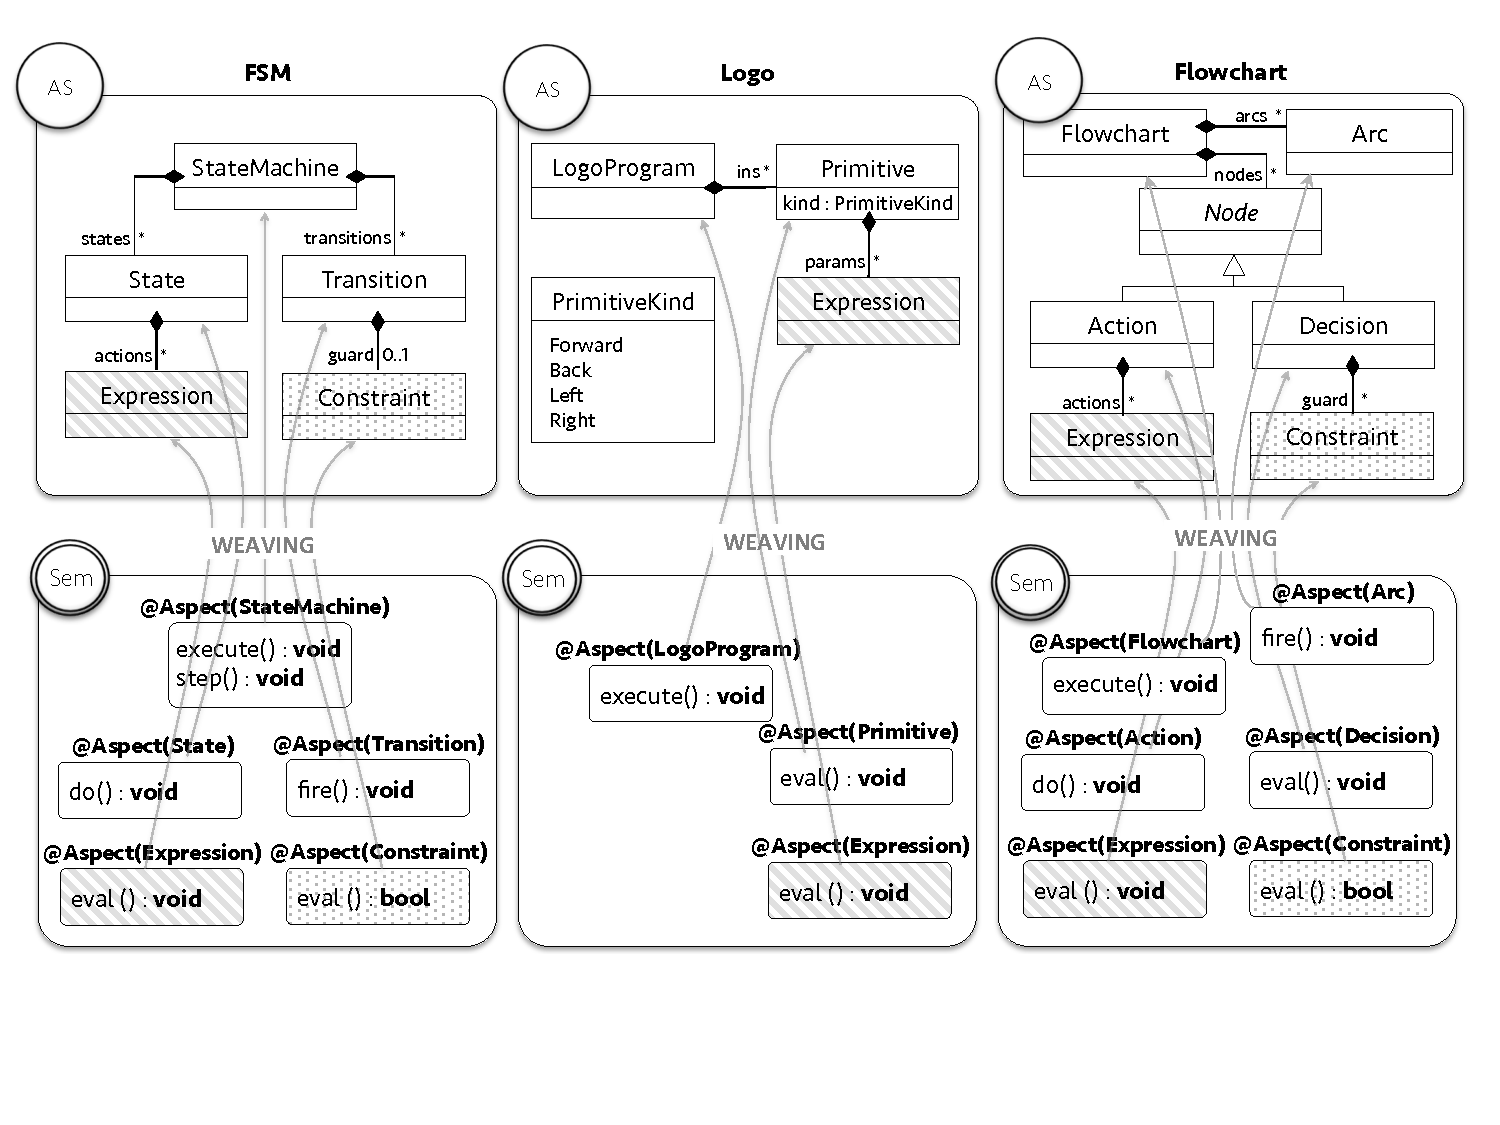
\includegraphics[width=1\linewidth]{images/domains-fig.pdf}
%\caption{Commonalities between domains and potential reuse}
%\label{fig:domains}
%\end{figure}

%Commonalities can be found between two ore more DSLs of the input set. That is, we can find metaclasses and domain specific actions that are shared by more than two DSLs. Hence, intersections should be searched among all the possible combinations of the DSLs in the input set. Once those functions are defined and implemented, the second phase is to use them in order to find the intersections among the DSLs of the input set. 



%there are three DSLs DSLs that are totally independent. That means that they do not share any of their language constructs, and consequently, there is not potential reuse between them. Differently, the two DSLs shown at the right of the figure have overlapping domains. That means that there are a subset of language that are \large\textbf{``equal'' }\normalsize in both DSLs. Note that if two language constructs are the same, we can assume that their specifications are equal and can be reused instead of being replicated.




%Moreover, there are set of DSLs for which the domains can be hierarchically organized \cite[p. 60-61]{voelter:2013}.

%\subsection{Equivalence between language constructs}

%So far, we have based the notion of potential reuse in DSLs on the commonalities existing in a set of DSLs. Nevertheless, this assumption supposes that we are able to compare two language constructs in order to know if they are equivalent. So, now we need to define this \textit{equivalence} relationship. In particular, the comparison of two language constructs relies on two dimensions: (1) comparison of the meta-classes in the abstract syntax; and (2) comparison of the domain-specific actions in the semantics.

